\documentclass[11pt,a4paper]{article}

\usepackage[margin=1in]{geometry}
\usepackage{amsmath}
\usepackage{graphicx}
\usepackage{booktabs}
\usepackage{url}
\usepackage{listings}
\usepackage{xcolor}
\usepackage{enumitem}
\usepackage[most]{tcolorbox}

\lstset{
    language=Python,
    basicstyle=\ttfamily\footnotesize,
    numbers=left,
    numberstyle=\tiny,
    numbersep=8pt,
    breaklines=true,
    columns=fullflexible,
    keepspaces=true,
    showstringspaces=false,
    frame=single
}

\title{Homework Report: Real and Simulated Time Series}
\author{Anton Henkel, Alessandro Comencini, Erik Soehner}
\date{\today}

% Writing aids, to be replaced by our own text:
% - In the PDF: a yellow "Example skeleton" box per paragraph, one possible order of points.
% - Only here in the source: NOTES (key results, possible interpretations) and
%   NARRATION IDEAS (how the section could tell its story) as comments above each box.
% Delete the comments and the skeleton box once a paragraph is written.
\definecolor{skeleton}{rgb}{0.6,0.45,0}
\newtcolorbox{skeletonbox}{breakable, enhanced, colback=yellow!10, colframe=skeleton, boxrule=0.6pt, arc=2pt,
  left=6pt, right=6pt, top=4pt, bottom=4pt, fonttitle=\bfseries, coltitle=white, title={Example skeleton (replace with own text)}}
\newenvironment{skeleton}{\begin{skeletonbox}\begin{enumerate}[label=\arabic*., leftmargin=*, itemsep=5pt, topsep=0pt]}{\end{enumerate}\end{skeletonbox}}
\setlist[itemize]{topsep=1pt, itemsep=0pt, parsep=0pt}

\begin{document}

\maketitle
\thispagestyle{empty}

\setcounter{page}{1}

\section{Domains and Their Time Series}

% NOTES:
% - Lecture vocabulary \cite{lecture-ts}: trend, seasonal, random component; additive $X_t = T_t + S_t + R_t$ vs.\ multiplicative $X_t = T_t \cdot S_t \cdot R_t$; autocorrelation.
% - Figure~\ref{fig:decomposition}: robust STL \cite{cleveland-stl}, period 12. Robust variant: isolated events go into the random part instead of distorting trend/seasonal.
% NARRATION IDEAS:
% - Open with the lens: we look at both domains through the lecture's three components, so the reader knows what to look for in every figure.
% - Say in one line why decomposition comes first: it tells us what a good simulation has to reproduce.
% - Optional: why robust STL instead of a plain decomposition (two obvious outliers in gym).
\begin{skeleton}
\item \textbf{How we look at a time series}
\begin{itemize}
  \item the three components from the lecture: trend, seasonal, random
  \item they can add up or multiply
\end{itemize}
\item \textbf{Why we start with a decomposition}
\begin{itemize}
  \item it shows what a good simulation has to reproduce
\end{itemize}
\item \textbf{Method}
\begin{itemize}
  \item robust STL with a 12-month period
  \item robust, so single unusual months do not distort trend and seasonality
  \item result in Figure~\ref{fig:decomposition}
\end{itemize}
\end{skeleton}

\begin{figure}[!htb]
\centering
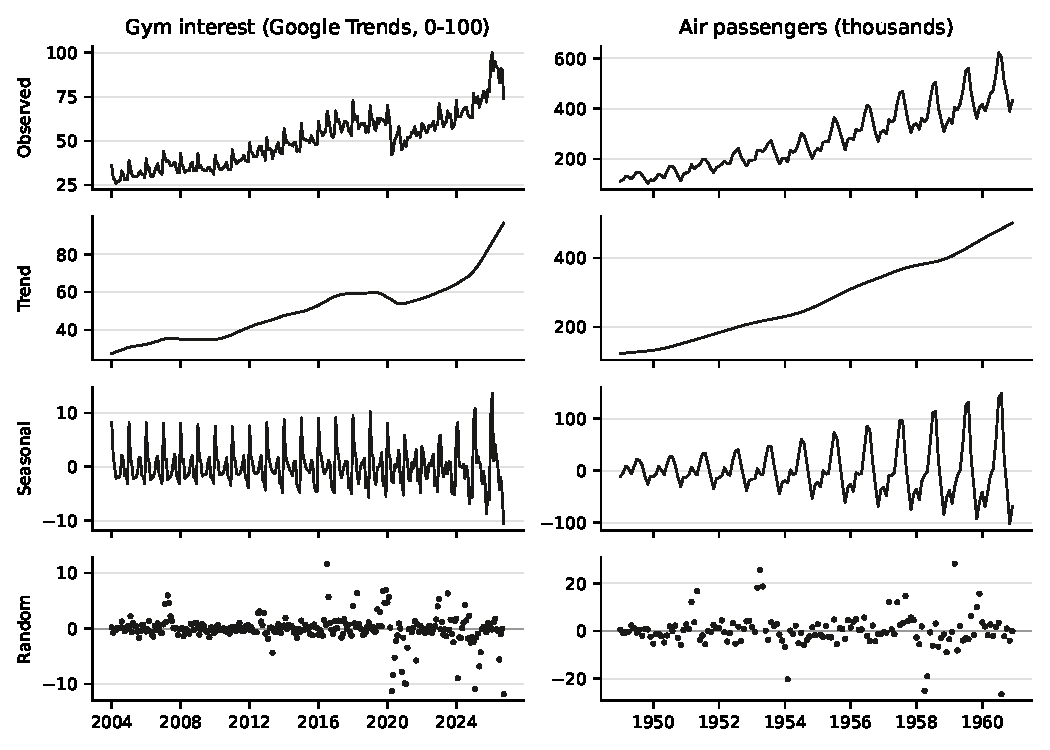
\includegraphics[width=0.6\textwidth]{figures/stl_decomposition.pdf}
\caption{Robust STL decomposition of the real series into trend, seasonal, and random components.}
\label{fig:decomposition}
\end{figure}

\subsection{Gym Interest}

% NOTES:
% - Source \cite{google-trends-gym}: Google Trends, search term ``gym'', worldwide, monthly, Jan 2004 -- Oct 2026, 274 months. Relative scale, 100 = month of peak interest, no absolute unit.
% - Trend: slow rise until 2019, drop 2020, steep rise from 2022.
% - Seasonal: peak January (+17\% vs.\ trend), New Year's resolutions? Low Oct--Dec, lowest December ($-8\%$) (Figure~\ref{fig:profile}). Small compared with the trend.
% - Random: spike July 2016 (coincides with Pok\'emon Go release, game locations are called ``gyms'', our interpretation); fall spring 2020 (COVID-19 gym closures).
% NARRATION IDEAS:
% - Lead with what the series measures and its catch (relative scale, no unit), then walk through trend $\to$ seasonal $\to$ random in the same order as the figure.
% - The events are the memorable part: one concrete sentence each makes the random component tangible.
% - Flag the Pok\'emon Go link as our reading (``coincides with''), not a proven cause.
\begin{skeleton}
\item \textbf{What the data is}
\begin{itemize}
  \item Google Trends interest in ``gym'', worldwide, monthly
  \item January 2004 to October 2026, 274 months
  \item relative scale: 100 is the month with the most searches, no real unit
\end{itemize}
\item \textbf{Trend}
\begin{itemize}
  \item slow rise until 2019
  \item drop in 2020
  \item steep rise from 2022
\end{itemize}
\item \textbf{Seasonal pattern}
\begin{itemize}
  \item highest in January, 17\% above the trend (New Year's resolutions?)
  \item lowest in December, 8\% below the trend
  \item small compared with the trend
\end{itemize}
\item \textbf{Random part}
\begin{itemize}
  \item spike in July 2016, same month as the Pok\'emon Go release (our guess)
  \item fall in spring 2020, gyms closed during COVID-19
\end{itemize}
\item \textbf{Main point}
\begin{itemize}
  \item the trend is driven by events, the seasonality is weak
\end{itemize}
\end{skeleton}

\subsection{Air Passengers}

% NOTES:
% - Source \cite{box-jenkins,selva86-airpassengers}: international airline passengers, thousands, monthly, Jan 1949 -- Dec 1960, 144 months (Box \& Jenkins Series G).
% - Trend: almost linear, about 120 $\to$ 470 thousand.
% - Seasonal: peak July/August (+22\%), low November ($-20\%$). Amplitude grows with the level $\Rightarrow$ multiplicative model.
% - Random: small, no isolated events.
% NARRATION IDEAS:
% - Same order as gym, so the two domains are easy to compare side by side.
% - Use it as the textbook contrast: steady trend, strong regular seasonality, little noise.
% - The growing seasonal swings are the visual argument for a multiplicative model; point the reader to where to see it in Figure~\ref{fig:decomposition}.
\begin{skeleton}
\item \textbf{What the data is}
\begin{itemize}
  \item international airline passengers in thousands, monthly
  \item January 1949 to December 1960, 144 months
\end{itemize}
\item \textbf{Trend}
\begin{itemize}
  \item almost a straight line, from about 120 to 470 thousand
\end{itemize}
\item \textbf{Seasonal pattern}
\begin{itemize}
  \item highest in July and August, 22\% above the trend
  \item lowest in November, 20\% below the trend
  \item the yearly swings get bigger as the series grows, so the components multiply
\end{itemize}
\item \textbf{Random part}
\begin{itemize}
  \item small, no unusual months
\end{itemize}
\item \textbf{Main point}
\begin{itemize}
  \item the opposite of gym: regular and predictable
\end{itemize}
\end{skeleton}

\section{Simulation}

% NOTES:
% - Course generator (Moodle) only runs on Windows; nobody in the group has a Windows machine $\Rightarrow$ model-based generator instead.
% - Holt-Winters, statsmodels \cite{seabold-statsmodels}: additive trend, multiplicative seasonality (matches Figure~\ref{fig:decomposition}), period 12. Fitted to each real series.
% - 10 simulations per domain, same length as the real series, start from the fitted initial state, random multiplicative errors, seed 42.
% - Table~\ref{tab:params}. Gym: $\alpha = 0.63$ high $\Rightarrow$ level follows the series closely, changes treated as permanent; $\gamma = 0$ $\Rightarrow$ fixed seasonal pattern. Air: $\gamma = 0.60$ $\Rightarrow$ seasonal pattern updated strongly, amplitude can grow with the level. $\beta = 0$ for both.
% NARRATION IDEAS:
% - Start with the honest constraint (Windows-only tool) and turn it into a choice: a generator that learns its parameters from the data.
% - Connect the model choice back to Section~1: multiplicative seasonality because the decomposition showed it.
% - Don't explain every parameter; translate only $\alpha$ and $\gamma$ into plain words, since the later sections rely on them.
\begin{skeleton}
\item \textbf{Why not the course tool}
\begin{itemize}
  \item the Moodle generator only runs on Windows
  \item nobody in the group has a Windows machine
\end{itemize}
\item \textbf{What we used instead}
\begin{itemize}
  \item Holt-Winters model in Python (statsmodels)
  \item it learns its parameters from the real series
\end{itemize}
\item \textbf{Model setup}
\begin{itemize}
  \item growing trend, seasonality that scales with the level, 12-month period
  \item matches what the decomposition showed
\end{itemize}
\item \textbf{How we simulated}
\begin{itemize}
  \item 10 series per domain, same length as the real one
  \item each starts where the fitted model starts
  \item random noise added, fixed seed so it can be repeated
\end{itemize}
\item \textbf{What the parameters mean (Table~\ref{tab:params})}
\begin{itemize}
  \item gym: the level follows the real series closely, the seasonal pattern never changes
  \item air: the seasonal pattern keeps adapting, so its swings can grow
\end{itemize}
\end{skeleton}

\begin{table}[!htb]
\centering
\small
\begin{tabular}{lrrrrr}
\toprule
Domain & $\alpha$ (level) & $\beta$ (trend) & $\gamma$ (seasonal) & Initial level & Relative residual s.d. \\
\midrule
Gym & 0.63 & 0.00 & 0.00 & 29.3 & 5.0\% \\
Air & 0.32 & 0.00 & 0.60 & 124.7 & 3.8\% \\
\bottomrule
\end{tabular}
\caption{Fitted Holt-Winters parameters. A value of 0 means the component is fixed after initialisation.}
\label{tab:params}
\end{table}

\section{Real and Simulated Series}

\begin{figure}[!htb]
\centering
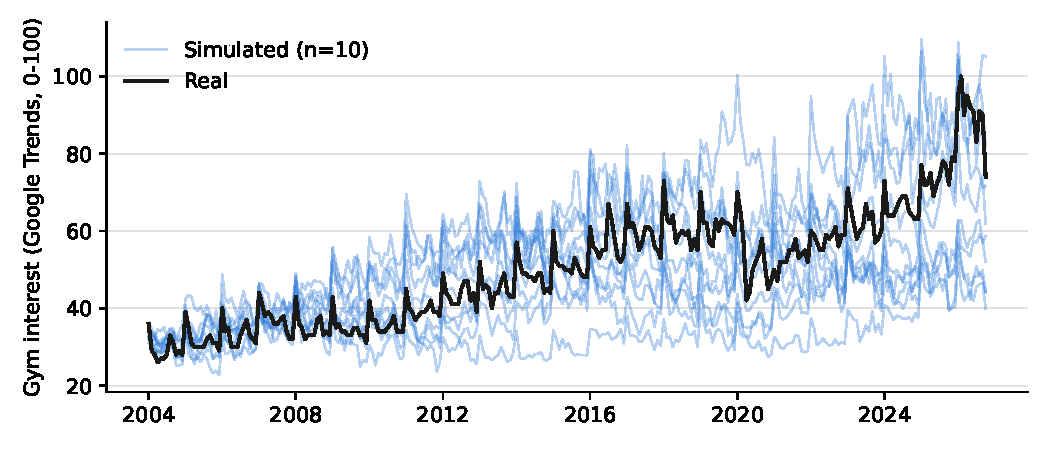
\includegraphics[width=0.62\textwidth]{figures/gym_real_vs_simulated.pdf}
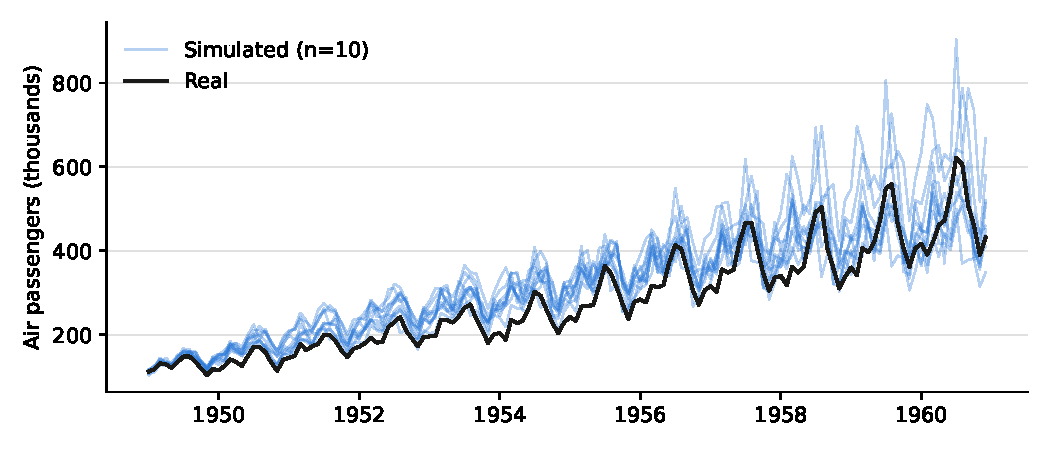
\includegraphics[width=0.62\textwidth]{figures/air_real_vs_simulated.pdf}
\caption{Real series (black) and 10 Holt-Winters simulations (blue) for gym interest (top) and air passengers (bottom).}
\label{fig:simulated}
\end{figure}

% NOTES:
% - Figure~\ref{fig:simulated}, air: simulations stay close, reproduce trend and growing seasonal swings.
% - Gym: simulations spread out over time, range about 40 to over 100 by 2026; none shows the 2020 fall or the rise after 2022.
% - Detrended comparison (divide by 12-month moving average), figures in Appendix~\ref{app:figures}:
%   gym: seasonal profile (Figure~\ref{fig:profile}) and autocorrelation (Figure~\ref{fig:acf}) match almost exactly (fixed seasonal pattern, $\gamma = 0$);
%   air: seasonal pattern blurred, summer peak +14\% instead of +22\%, extra peak in March; lag-1 autocorrelation 0.35 (simulated mean) vs.\ 0.67 (real) $\Rightarrow$ real deviations from the trend last longer.
% - Possible interpretation: both air effects come from $\gamma = 0.60$, the simulated seasonal pattern changes randomly from year to year instead of smoothly.
% NARRATION IDEAS:
% - Lead with the visual impression of Figure~\ref{fig:simulated} (air: tight bundle; gym: fan that opens up), then go below the surface.
% - Frame the appendix analysis as a question: does the model get the seasonal and random structure right once the trend is removed?
% - Nice twist to build towards: each domain fails in a different place (gym: trend, air: seasonality).
\begin{skeleton}
\item \textbf{First impression (Figure~\ref{fig:simulated})}
\begin{itemize}
  \item air: simulations stay close to the real series
  \item gym: simulations spread out more and more over time
\end{itemize}
\item \textbf{What gym misses}
\begin{itemize}
  \item by 2026 the simulations range from about 40 to over 100
  \item none shows the 2020 drop or the rise after 2022
\end{itemize}
\item \textbf{Looking closer, without the trend}
\begin{itemize}
  \item each series divided by its 12-month average
  \item figures in the appendix
\end{itemize}
\item \textbf{Gym without the trend}
\begin{itemize}
  \item seasonal pattern and month-to-month correlation match the real series almost exactly
\end{itemize}
\item \textbf{Air without the trend}
\begin{itemize}
  \item summer peak too low: 14\% instead of 22\% above the trend
  \item an extra peak in March that the real series does not have
  \item deviations from the trend fade faster than in the real series
\end{itemize}
\item \textbf{Why}
\begin{itemize}
  \item the model lets the air seasonal pattern change randomly every year
\end{itemize}
\item \textbf{Main point}
\begin{itemize}
  \item each domain goes wrong in a different place: gym in the trend, air in the seasonality
\end{itemize}
\end{skeleton}

\section{Distances Between Series}

% NOTES:
% - Two measures from the lecture \cite{lecture-ts}: Euclidean (point by point at the same time) and DTW (aligns the series first, tolerates time shifts).
% - z-normalisation first: otherwise between-domain distances mostly measure scale (0--100 vs.\ thousands), not shape.
% - Euclidean needs equal length $\Rightarrow$ all series cut to the last 144 months (gym: Nov 2014 -- Oct 2026). DTW on the same window for comparability.
% - 11 series per domain (1 real + 10 simulated) $\Rightarrow$ 55 pairs within a domain, 121 between.
% NARRATION IDEAS:
% - Present each method choice as the answer to a problem: different scales $\to$ normalise; different lengths $\to$ common window; time shifts $\to$ DTW.
% - Tie the two measures to the lecture explicitly (alignment problem of Euclidean distance).
\begin{skeleton}
\item \textbf{Two ways to measure distance (from the lecture)}
\begin{itemize}
  \item Euclidean: compares the values month by month
  \item DTW: lines the series up first, so small time shifts do not count
\end{itemize}
\item \textbf{Problem: different scales}
\begin{itemize}
  \item gym 0 to 100, air in thousands
  \item each series rescaled to mean 0 and spread 1, so only the shape counts
\end{itemize}
\item \textbf{Problem: different lengths}
\begin{itemize}
  \item all series cut to the last 144 months
  \item for gym that is November 2014 to October 2026
  \item DTW uses the same months, so both measures are comparable
\end{itemize}
\item \textbf{What we compare}
\begin{itemize}
  \item 11 series per domain: 1 real, 10 simulated
  \item results in Table~\ref{tab:distances}
\end{itemize}
\end{skeleton}

\begin{table}[!htb]
\centering
\small
\begin{tabular}{lrrr}
\toprule
Comparison & Pairs & Euclidean & DTW \\
\midrule
Within gym (all series) & 55 & 12.4 & 73.2 \\
Within air (all series) & 55 & 4.1 & 26.1 \\
Gym: real vs.\ simulated & 10 & 10.7 & 64.3 \\
Air: real vs.\ simulated & 10 & 4.1 & 26.4 \\
Gym vs.\ air (all series) & 121 & 12.6 & 78.0 \\
Gym vs.\ air (real series only) & 1 & 9.8 & 47.5 \\
\bottomrule
\end{tabular}
\caption{Mean distances between z-normalised series over the last 144 months.}
\label{tab:distances}
\end{table}

% NOTES:
% - Air: real vs.\ simulated (4.1) as close as simulations among themselves (4.1) $\Rightarrow$ domain captured well.
% - Gym: about 3$\times$ further apart; real gym is closer to real air (9.8) than to its own simulations (10.7).
% - Possible interpretation: after normalisation both real series are ``upward trend + yearly seasonality''; gym simulations drift during the decade before the comparison window.
% - DTW: lower values, same ranking as Euclidean.
% NARRATION IDEAS:
% - Lead with the surprising result: real gym is closer to real air than to its own simulations.
% - Then explain it: after normalisation, shape is what counts, and the gym simulations lose the shape over time.
% - Keep DTW to one sentence, it only confirms the ranking.
\begin{skeleton}
\item \textbf{Surprising result first}
\begin{itemize}
  \item the real gym series is closer to the real air series than to its own simulations
\end{itemize}
\item \textbf{Air}
\begin{itemize}
  \item real series as close to the simulations as they are to each other
  \item so the simulation fits this domain well
\end{itemize}
\item \textbf{Gym}
\begin{itemize}
  \item distances about three times larger than for air
\end{itemize}
\item \textbf{Why}
\begin{itemize}
  \item after rescaling, both real series look alike: rising trend plus yearly pattern
  \item the gym simulations drift away during the ten years before the compared window
\end{itemize}
\item \textbf{DTW}
\begin{itemize}
  \item smaller numbers, but the same ranking as Euclidean
\end{itemize}
\end{skeleton}

\section{Conclusions}

% NOTES:
% - Required by the task: how well the series were simulated, pros and cons of the tool.
% - How well: air captures the dominant steady trend, blurs seasonality; gym captures seasonality, not the trend (external events: Pok\'emon Go, pandemic; replaced by random drift in the simulations).
% - Whole-series distances mostly reflect the trend; seasonal profile and autocorrelation show the other components. Links to the lecture: comparing time series is domain dependent and depends on the measure \cite{lecture-ts}.
% - Pros of Holt-Winters as a generator: parameters estimated from data (not hand-set), reproducible (seed), any platform, any number of series.
% - Cons: only trend + seasonality + independent errors $\Rightarrow$ no events or structural breaks; no domain knowledge: 3 of 10 gym simulations exceed 100 (max.\ 110), impossible on the Trends scale.
% NARRATION IDEAS:
% - Answer the task's two questions directly, in this order: how well simulated, then pros and cons.
% - One sentence per domain is enough; refer back instead of repeating numbers.
% - End on the general lesson (what you find depends on how you compare) or on the most concrete con (simulated gym values above 100).
\begin{skeleton}
\item \textbf{How well were the series simulated?}
\begin{itemize}
  \item air: trend well, seasonal pattern blurred
  \item gym: seasonal pattern well, trend not, because a model cannot foresee events like Pok\'emon Go or the pandemic
\end{itemize}
\item \textbf{What we learned}
\begin{itemize}
  \item the answer depends on how you compare
  \item whole-series distances mostly see the trend, the seasonal profile sees the rest
  \item fits the lecture: comparing time series depends on the domain and the measure
\end{itemize}
\item \textbf{Pros of the tool}
\begin{itemize}
  \item parameters come from the data, not guessed by hand
  \item repeatable, runs on any computer, as many series as needed
\end{itemize}
\item \textbf{Cons of the tool}
\begin{itemize}
  \item cannot create events or sudden breaks
  \item knows nothing about the domain: some gym simulations go above 100, which Google Trends never does
\end{itemize}
\end{skeleton}

\section{Use of AI}

% NOTES:
% - Check the course's AI policy on Moodle first; adapt the statement below so it is accurate for what we actually did.
% - Suggested statement: ``We used an AI assistant (Claude, Anthropic) to summarise the lecture slides, to help write and debug the Python scripts for simulation, figures and distances, and to propose an outline with key results for this report. We checked the code and all numbers ourselves. The text of the report was written by us; the AI assistant was used for language checks only.''
% NARRATION IDEAS:
% - Keep it short, factual and specific: tools, what for, what we checked ourselves.
\begin{skeleton}
\item \textbf{Which tool}
\begin{itemize}
  \item Claude (Anthropic)
\end{itemize}
\item \textbf{What it was used for}
\begin{itemize}
  \item summarising the lecture slides
  \item writing and debugging the Python scripts
  \item proposing an outline with key results
  \item checking language
\end{itemize}
\item \textbf{What we did ourselves}
\begin{itemize}
  \item writing the text
  \item checking the code and all numbers
\end{itemize}
\item \textbf{Before submitting}
\begin{itemize}
  \item check the course rules on Moodle
\end{itemize}
\end{skeleton}

\nocite{*}
\bibliographystyle{plain}
\bibliography{bibliography}

\appendix
\section{Seasonal Profile and Autocorrelation}
\label{app:figures}

\begin{figure}[h]
\centering
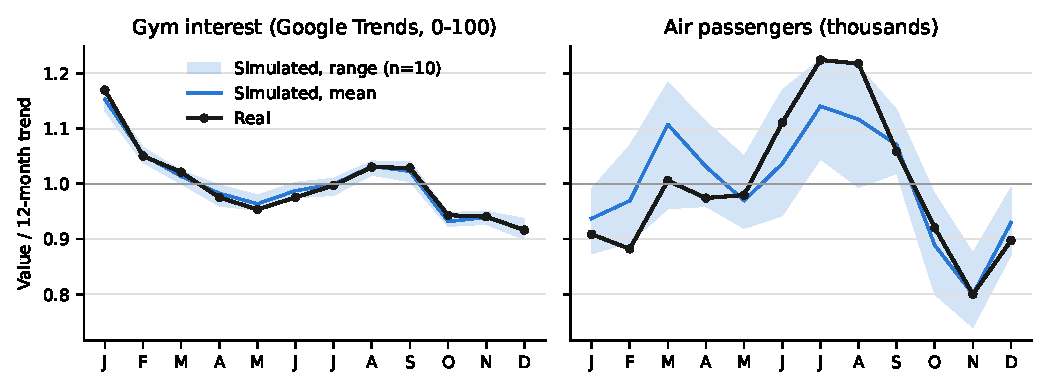
\includegraphics[width=0.72\textwidth]{figures/seasonal_profile.pdf}
\caption{Average value per calendar month relative to the 12-month trend, real series against the range and mean of the simulations.}
\label{fig:profile}

\vspace{1ex}
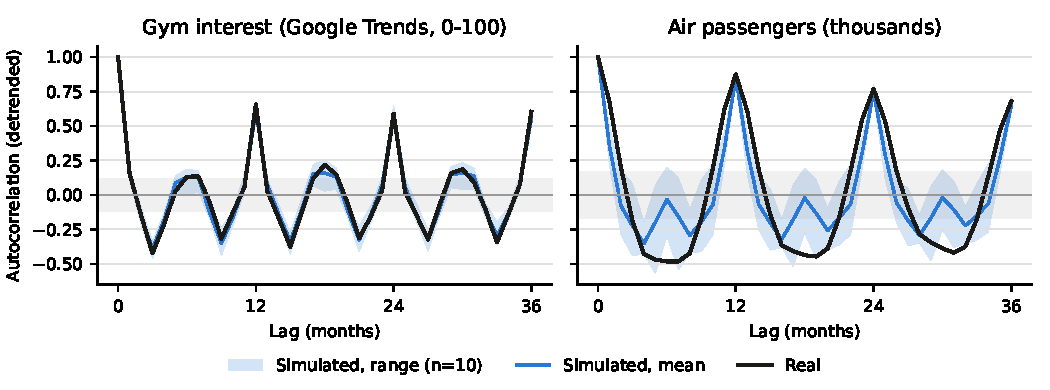
\includegraphics[width=0.72\textwidth]{figures/acf_real_vs_simulated.pdf}
\caption{Autocorrelation of the detrended series up to 36 months. The grey band marks values compatible with no autocorrelation.}
\label{fig:acf}
\end{figure}

\end{document}
